\subsection{Temporal patterns and indexing} \label{tpatterns}
In previous sections of this chapter I have shown the PAA and SAX algorithms for conversion of real valued time series into the symbolic representation along with symbolic temporal data models, concepts and operators. All of this is a necessary background in order to understand approaches for unsupervised knowledge mining from a symbolic temporal data. In this section I will review sequential pattern mining algorithms from time points and time-intervals data. I will focus the review on the univariate data then extending it to the multivariate.

Before discussing algorithms, I need to provide a formal definition of \textit{pattern}. The essential property which defines a pattern is called \textit{support}. Support, roughly speaking, is the frequency of occurrence of a certain pattern in the observed data. It is generally assumed that each of the possible patterns have a certain probability to be seen in the dataset just by chance, and this probability is called the \textit{expected} probability and defines the \textit{expected support} for the pattern. When the actual observed support (or frequency) of a pattern significantly differs from the expected one, it is called \textit{significant support} and indicates that pattern might have some meaningful knowledge artifact attached to it. Although support different from the expected level does not guarantee usefulness or interestingness, it is used for a powerful pruning of a search space since most possible patterns will not have sufficient support. Note, that there is an other property \cite{citeulike:2804633} discussed in the literature which essentially similar to support: \textit{confidence}. Usually confidence correlates with support, i.e. greater support corresponds to higher confidence.

There are two well-established categories of patterns with significant support. The first category of patterns, frequently occurring ones (with support higher than expected), is very important in many data mining areas such as medicine, motion-capture, robotics, video surveillance, meteorology and others. Patterns from this category usually named as \textit{repeated}, \textit{approximately repeated} or \textit{motifs}. The second category of patterns, contains patterns with the support lower than expected, this type of pattern is named \textit{surprise} or \textit{novelty} patterns. Novelty patterns also have a great value for many applications: for example it is important to detect unusual semi-repeated pattern in the ECG data diagnosing heartbeat abnormalities, or detecting unusual activity patterns in video surveillance recognizing a suspicious activity.

The temporal motif finding problem from symbolic data is very similar to one of the central problems in the field of Computational Biology \cite{citeulike:465665}. Many algorithms are very similar, but, in Biology, motifs are usually \textit{informative} and bear some information about evolutionary artifacts, which is not true in the field of time-series analysis \cite{citeulike:3978085}.

\subsection{Time points patterns}
According to M\"orchen, the most commonly searched pattern within univariate symbolic time series is order. This search for a particular order of symbols within a subsequence is called \textit{sequential pattern mining} \cite{citeulike:775528} and does not necessarily require symbols to be consecutive.

\begin{figure}[tbp]
   \centering
   \includegraphics[height=55mm]{time-points.eps}
   \caption{The time-points patterns as explained in \cite{citeulike:1748833}}
   \label{fig:timepoints}
\end{figure}

The classical suffix tree algorithm \cite{citeulike:707616} with some modifications is a standard approach for pattern discovery from string time-series according to Palopoli et al. \cite{citeulike:5003338}. In this paper, the authors discuss algorithms for automatic discovery of frequent patterns (\textit{motifs}) in ``exact'' or ``approximate'' forms. There are two approaches generally used for the suffix tree building: \textit{generative}, when algorithms generate all possible patterns and test their appearance frequency \cite{citeulike:5012661}, and \textit{scanning}, when a sliding window used to scan over the sequences available and construct the tree on the fly \cite{citeulike:5012661}. In \cite{citeulike:5003404} Jiang \& Hamilton compare traversal strategies for suffix trees: breadth-first ($BF$, $O(K^{2}n)$), depth-first ($DF$, $O(Kn)$) and the heuristic depth-first (HDF) algorithms implementations for temporal data mining.

The limitation of the suffix-tree based algorithms is that the maximum length of a pattern needs to be specified upon tree construction since all sub-sequences of this length are generated or extracted from the time series with a sliding window.

Another approach, specifically designed for the \textit{surprise pattern} finding problem, is proposed by Keogh et al. in \cite{citeulike:3025877}. The authors discuss methods for finding a surprise pattern from the temporal data and propose their ``TARZAN'' algorithm which is based upon suffix tree and Markov model, reporting surprising patterns occurring with a frequency substantially different from that expected by chance.

\subsection{Time interval patterns}
As we saw before, the duration concept is implicit in the time interval definition. Nevertheless, while defining a time-interval pattern we do not actually take into account the length of the interval. Interval relations are abstracted to the ``border'' or ``mean points'' relations.

\textit{Containment patterns} are discussed by Villafane et al. in \cite{citeulike:2804633}. This type of temporal patterns has found application to many areas, for example software system log mining. In this case it is important to see what events were happening within the resource overload time interval. Another example is medicine: what was happening with the heartbeat within the period when patient's fever was high? The authors propose a method based on \textit{containment graphs} which allows counting of the containment frequency based on a lattice. The authors designed a naive algorithm of the graph traversal performed incrementally by the path-size and have shown satisfiable results considering their limitations in computational power. One of the limitations found is that it yields different patterns describing the same temporal events. An example of containment patterns is shown at Figure \ref{fig:timeintervals} panel \textit{a}, this figure is borrowed from \cite{citeulike:1748833}.

\begin{figure}[tbp]
   \centering
   \includegraphics[height=75mm]{time-intervals.eps}
   \caption{The time-interval patterns from \cite{citeulike:1748833}}
   \label{fig:timeintervals}
\end{figure}

Allen's relations are used in many of the approaches to mining of time-interval patterns. In \cite{citeulike:5159362}, Kam \& Fu considered interval-based events where duration is expressed in terms of end-points relations and designed a category of \textit{A1} temporal patterns based on Allen's relations. However, Kam and Fu restrict the search space to the right concatenations of intervals corresponding to existing patterns and limit the depth of the patterns. Depending on time-interval consideration order, this approach yields different patterns describing same events, for example on the Figure \ref{fig:timeintervals} panel \textit{b}: left pattern is \textit{(((A starts B) overlaps C) overlaps D)} whether right one is \textit{(((A before C) started by B) overlaps D)}.

\textit{Fluents}, another type of time-interval patterns based on the Allen's algebra, were introduced by Cohen in \cite{citeulike:5153756} to address the problem of unsupervised learning of structures in time series. The formal definition given by the authors states that ``Fluents are logical descriptions of situations that persist, and composite fluents are statistically significant temporal relationships between fluents.'' Sliding window and Apriori algorithms are used in this work. The \textit{Fluent learning algorithm} designed by the authors was applied to the robot motion data collected by sensors and helped in the discovery of temporal patterns indicating persistent robot behavior along with problems with robot's sonar system. This algorithm suffers from the same problem as A1 - it reports variations of the same pattern as different patterns. The authors had to remove ``the set of variants'' manually before presenting results.

H\"{o}ppner, in \cite{citeulike:5159615}, demonstrates an approach to association rules mining through the use of \textit{state sequences}. State sequences based on pairwise relations between all temporal intervals according to Allen. A sliding window is used to generate sub-sequences and the duration of the pattern over consecutive sliding windows is used to quantify the pattern support value. This information is then used in the Apriori algorithm for pattern discovery. The experimental validation of the algorithm on the weather dataset shows the ability of the approach to yield meaningful patterns.

$UTG$ relations were used in some work for temporal interval patterns mining (Figure \ref{fig:timeintervals} panel \textit{d}), but according to M\"orchen \cite{citeulike:1748833}, it was ``criticized for the strict conditions relating interval boundaries''. UTG rules place restrictions on the intervals, requiring the start and end of the intervals in the pattern to be almost simultaneous. Also, lacking the ability to express the concept of coincidence, UTG-based methods found somewhat limited application. However, Guimar\~{a}es in \cite{citeulike:5159924} shows targeted application of UTG-based linguistic knowledge representation to the discovery of sleep-related breathing disorders. Results of this study  allowed doctors to improve diagnosis, and moreover, led to the discovery of previously unknown recurrent behaviors among patients.

Unlike UTG, $TSKR patterns$ provide support for a partial order and allow inclusion of the sub-intervals into the pattern. This makes them more expressive than UTG and Allen's relations. \textit{TSKR Chord} patterns shown at the Figure \ref{fig:timeintervals} panel \textit{e} are mined with the CHARM \cite{citeulike:769773} algorithm extended with a support function that counts the duration of the pattern occurrence \cite{citeulike:1748833}. \textit{TSKR Phrase} patterns, in turn, are built upon the partial order of the several Chords (\ref{fig:timeintervals} panel \textit{f}), and provide greater sensitivity and selectivity for temporal patterns mining.
